\documentclass[tikz,border=2mm]{standalone}
\usetikzlibrary{3d,perspective}

\tikzset
{
	my rectangle/.style={dotted,fill=white,fill opacity=0.5},
	my node/.style={circle,draw,shading=ball,ball color=orange}
}
% Code from https://tex.stackexchange.com/questions/637125/how-to-draw-book-embeddings-with-tikz
\begin{document}
	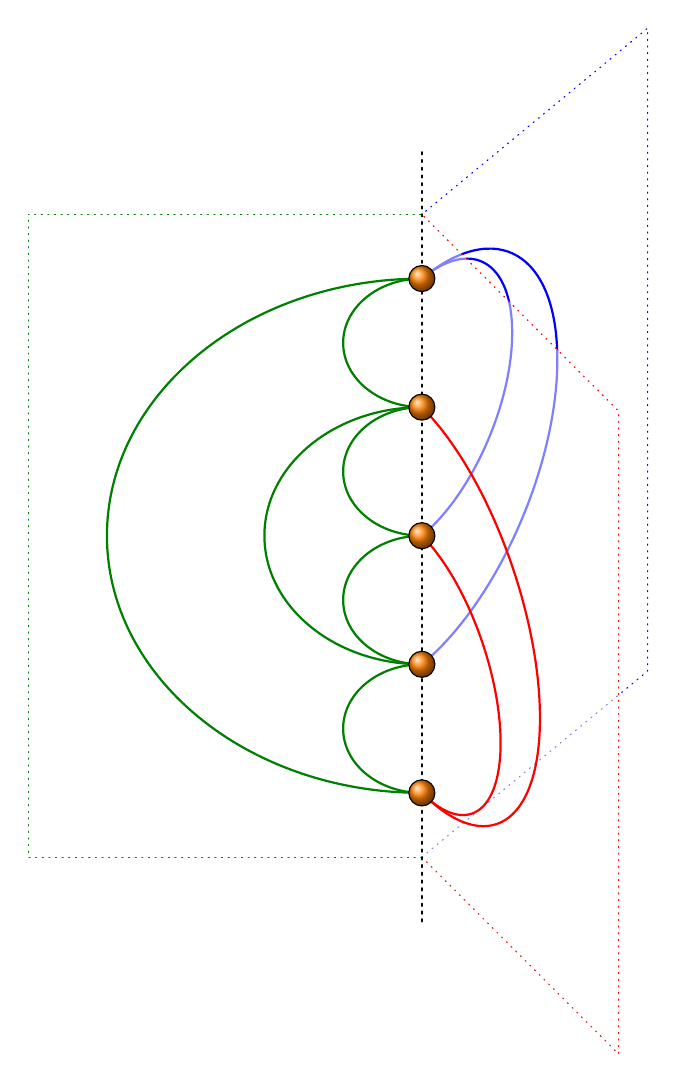
\begin{tikzpicture}[isometric view,line cap=round,line join=round]
		% coordinates
		\foreach[count=\j]\i in {1,3,5,7,9}
		\coordinate (\j) at (0,0,\i);
		% blue plane
		\begin{scope}[rotate around z=10,canvas is xz plane at y=0,blue]
			\draw[my rectangle] (0,0) -| (5,10) -- (0,10);
			\foreach\i in {2,3}
			\draw[thick] (\i) arc (-90:90:5-\i);
		\end{scope}
		% green plane
		\begin{scope}[rotate around z=135,canvas is xz plane at y=0,,green!50!black]
			\draw[my rectangle] (0,0) -| (5,10) -- (0,10);
			\foreach\i in {1,2,3,4}
			\pgfmathsetmacro\j{\i+1}
			\draw[thick] (\i) arc (-90:90:1);
			\draw[thick] (1) arc (-90:90:4);
			\draw[thick] (2) arc (-90:90:2);
		\end{scope}
		% red plane
		\begin{scope}[rotate around z=255,canvas is xz plane at y=0,red]
			\draw[my rectangle] (0,0) -| (5,10) -- (0,10);
			\foreach\i in {2,3}
			\draw[thick] (1) arc (-90:90:\i);
		\end{scope}
		% nodes / balls
		\draw[dotted,thick] (0,0,-1) -- (0,0,11);
		\foreach\i in {1,...,5}
		\node[my node] at (\i) {};
	\end{tikzpicture}
\end{document}